\documentclass[openany]{book}

\usepackage[margin=1in]{geometry}
\usepackage{amsmath,amsfonts,amsthm, amssymb}
\usepackage{yhmath}
\usepackage{mathrsfs}
\usepackage{mathtools}
\usepackage{xcolor}
\usepackage{graphicx}
\usepackage{comment}
\usepackage{tikz-cd}
\usepackage{quiver}
\renewcommand{\familydefault}{ppl}
\newcommand{\tr}{\text{tr}}
\newcommand{\R}{\mathbb{R}}
\newcommand{\E}{\mathbb{E}}
\newcommand{\Z}{\mathbb{Z}}
\newcommand{\C}{\mathbb{C}}
\newcommand{\F}{\mathbb{F}}
\newcommand{\la}{\langle}
\newcommand{\ra}{\rangle}
\newcommand{\colim}{\text{colim}}
\DeclareMathOperator{\im}{im}
\let\oldemptyset\emptyset
\let\emptyset\varnothing
\newcommand{\tor}{\text{Tor}}
\newcommand{\id}{\text{id}}
\newcommand{\ext}{\text{Ext}}
\newcommand{\ptop}{\text{PTop}}
\newcommand{\pt}{\text{pt}}
\newcommand{\ach}{\text{Ach}}
\newcommand{\Q}{\mathbb{Q}}
\newcommand{\gal}{\text{Gal}}


\usepackage{thmtools,thm-restate}

% Fixing mdframed skip below
% See https://tex.stackexchange.com/a/292090/143086
\usepackage[framemethod=TikZ]{mdframed}
\usepackage{xpatch}
\makeatletter
\xpatchcmd{\endmdframed}
	{\aftergroup\endmdf@trivlist\color@endgroup}
	{\endmdf@trivlist\color@endgroup\@doendpe}
	{}{}
\makeatother

\definecolor{huilightpink}{HTML}{fff2fe}
\definecolor{huidarkpink}{HTML}{d955b7}
\declaretheoremstyle[
	mdframed={
		backgroundcolor=huilightpink,
		linecolor=huidarkpink,
		rightline=false,
		topline=false,
		bottomline=false,
		linewidth=2pt,
		innertopmargin=5pt,
		innerbottommargin=8pt,
		innerleftmargin=8pt,
		leftmargin=-2pt,
		skipbelow=2pt,
		nobreak
	},
	headfont=\normalfont\bfseries\color{huidarkpink}
]{huipinkbox}
\declaretheorem[style=huipinkbox,name=Theorem,within=chapter]{thm}
\declaretheorem[style=huipinkbox,name=Theorem,sibling=thm]{theorem}




\begin{comment}
\definecolor{huilightyellow}{HTML}{fff5d6}
\definecolor{huidarkyellow}{HTML}{fcad03}
\declaretheoremstyle[
	mdframed={
		backgroundcolor=huilightyellow,
		linecolor=huidarkyellow,
		rightline=false,
		topline=false,
		bottomline=false,
		linewidth=2pt,
		innertopmargin=5pt,
		innerbottommargin=8pt,
		innerleftmargin=8pt,
		leftmargin=-2pt,
		skipbelow=2pt,
		nobreak
	},
	headfont=\normalfont\bfseries\color{huidarkyellow}
]{huiyellowbox}
\declaretheorem[style=huiyellowbox,name=Proposition,within=chapter]{prop}
\end{comment}



\definecolor{huilightpurple}{HTML}{faf2ff}
\definecolor{huidarkpurple}{HTML}{912ed9}
\declaretheoremstyle[
	mdframed={
		backgroundcolor=huilightpurple,
		linecolor=huidarkpurple,
		rightline=false,
		topline=false,
		bottomline=false,
		linewidth=2pt,
		innertopmargin=5pt,
		innerbottommargin=8pt,
		innerleftmargin=8pt,
		leftmargin=-2pt,
		skipbelow=2pt,
		nobreak
	},
	headfont=\normalfont\bfseries\color{huidarkpurple}
]{huipurplebox}
\declaretheorem[style=huipurplebox,name=Proposition,within=chapter]{prop}



% \definecolor{huilightpurple}{HTML}{faf2ff}
% \definecolor{huidarkpurple}{HTML}{912ed9}
% \declaretheoremstyle[
% 	mdframed={
% 		backgroundcolor=huilightpurple,
% 		linecolor=huidarkpurple,
% 		rightline=false,
% 		topline=false,
% 		bottomline=false,
% 		linewidth=2pt,
% 		innertopmargin=5pt,
% 		innerbottommargin=8pt,
% 		innerleftmargin=8pt,
% 		leftmargin=-2pt,
% 		skipbelow=2pt,
% 		nobreak
% 	},
% 	headfont=\normalfont\bfseries\color{huidarkpurple}
% ]{huipurplebox}
\declaretheorem[style=huipurplebox,name=Lemma,within=chapter]{lem}


\definecolor{lightpink}{HTML}{f0f6fc}
\definecolor{darkpink}{HTML}{2c72b8}
\declaretheoremstyle[
	mdframed={
		backgroundcolor=lightpink,
		linecolor=darkpink,
		rightline=false,
		topline=false,
		bottomline=false,
		linewidth=2pt,
		innertopmargin=5pt,
		innerbottommargin=8pt,
		innerleftmargin=8pt,
		leftmargin=-2pt,
		skipbelow=2pt,
		nobreak
	},
	headfont=\normalfont\bfseries\color{darkpink}
]{pinkbox}
\declaretheorem[style=pinkbox,name=Definition,within=chapter]{defn}


\definecolor{huilightblue}{HTML}{edf9ff}
\definecolor{huidarkblue}{HTML}{4b79db}
\declaretheoremstyle[
	mdframed={
		backgroundcolor=huilightblue,
		linecolor=huidarkblue,
		rightline=false,
		topline=false,
		bottomline=false,
		linewidth=2pt,
		innertopmargin=5pt,
		innerbottommargin=8pt,
		innerleftmargin=8pt,
		leftmargin=-2pt,
		skipbelow=2pt,
		nobreak
	},
	headfont=\normalfont\bfseries\color{huidarkblue}
]{huiblueblox}
\declaretheorem[style=huiblueblox,name=Example,within=chapter]{example}



% \definecolor{huilightblue}{HTML}{edf9ff}
% \definecolor{huidarkblue}{HTML}{4b79db}
% \declaretheoremstyle[
% 	mdframed={
% 		backgroundcolor=huilightblue,
% 		linecolor=huidarkblue,
% 		rightline=false,
% 		topline=false,
% 		bottomline=false,
% 		linewidth=2pt,
% 		innertopmargin=5pt,
% 		innerbottommargin=8pt,
% 		innerleftmargin=8pt,
% 		leftmargin=-2pt,
% 		skipbelow=2pt,
% 		nobreak
% 	},
% 	headfont=\normalfont\bfseries\color{huidarkblue}
% ]{huiblueblox}
% \declaretheorem[style=huiblueblox,name=Example,within=chapter]{example}

% \declaretheoremstyle[
% 	mdframed={
% 		backgroundcolor=huilightblue,
% 		linecolor=huidarkblue,
% 		rightline=false,
% 		topline=false,
% 		bottomline=false,
% 		linewidth=2pt,
% 		innertopmargin=5pt,
% 		innerbottommargin=8pt,
% 		innerleftmargin=8pt,
% 		leftmargin=-2pt,
% 		skipbelow=2pt,
% 		nobreak
% 	},
% 	headfont=\normalfont\bfseries\color{huidarkblue}
% ]{huiblueblox}
\declaretheorem[style=huiblueblox,name=Problem,within=chapter]{prob}



% \declaretheoremstyle[
% 	mdframed={
% 		backgroundcolor=huilightblue,
% 		linecolor=huidarkblue,
% 		rightline=false,
% 		topline=false,
% 		bottomline=false,
% 		linewidth=2pt,
% 		innertopmargin=5pt,
% 		innerbottommargin=8pt,
% 		innerleftmargin=8pt,
% 		leftmargin=-2pt,
% 		skipbelow=2pt,
% 		nobreak
% 	},
% 	headfont=\normalfont\bfseries\color{huidarkblue}
% ]{huiblueblox}
\declaretheorem[style=huiblueblox,name=Exercise,within=chapter]{exer}
\declaretheorem[style=huipinkbox, name=Corollary, within=chapter]{cor}





















\newcommand{\nirwarnsymbol}{%
	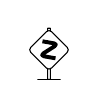
\begin{tikzpicture}[baseline=(x.base)]
		\draw[rounded corners=.01em] (-.05em,-1.07em)rectangle(.05em,.78em);
		\draw[fill=white,rounded corners=1.3] (0,.75em)--(.75em,0)--(0,-.75em)--(-.75em,0)--cycle;
		\draw[line width=0.2mm, line cap=round](-.4em,-1.07em)--(.4em,-1.07em);
		\node(x) at (0,0em) {};
		% Thank you https://tex.stackexchange.com/a/262510
		\draw[
			line cap=but,
			line join=round,
			x=.5em,
			line width=0.5mm,
			y=1*(height("Z")-\pgflinewidth)*(1-sin(10)),
			rotate=-10,
			rounded corners=1.5pt,
		](-0.57, 0.57) -- (0.57, 0.57) -- (-0.57, -0.57) -- (0.57, -0.57);
	\end{tikzpicture}%
}

%%%%%%%%%%%%%%%%%%%%%%%%%%%%%%%%%%%%%%%%%%%% MARGINS
\usepackage{marginnote}
% Thank you https://tex.stackexchange.com/a/472882
% Makes marginnotes always appear on the left, apparently
%
\makeatletter
\long\def\@mn@@@marginnote[#1]#2[#3]{%
	\begingroup
		\ifmmode\mn@strut\let\@tempa\mn@vadjust\else
			\if@inlabel\leavevmode\fi
			\ifhmode\mn@strut\let\@tempa\mn@vadjust\else\let\@tempa\mn@vlap\fi
		\fi
		\@tempa{%
			\vbox to\z@{%
				\vss
				\@mn@margintest
				\if@reversemargin\if@tempswa
						\@tempswafalse
					\else
						\@tempswatrue
				\fi\fi

					\llap{%
						\vbox to\z@{\kern\marginnotevadjust\kern #3
							\vbox to\z@{%
								\hsize\marginparwidth
								\linewidth\hsize
								\kern-\parskip
								%\mn@parboxrestore
								\marginfont\raggedleftmarginnote\strut\hspace{\z@}%
								\ignorespaces#1\endgraf
								\vss
							}%
							\vss
						}%
						\if@mn@verbose
							\PackageInfo{marginnote}{xpos seems to be \@mn@currxpos}%
						\fi
						\begingroup
							\ifx\@mn@currxpos\relax\else\ifx\@mn@currpos\@empty\else
									\kern\@mn@currxpos
							\fi\fi
							\ifx\@mn@currpage\relax
								\let\@mn@currpage\@ne
							\fi
							\if@twoside\ifodd\@mn@currpage\relax
									\kern-\oddsidemargin
								\else
									\kern-\evensidemargin
								\fi
							\else
								\kern-\oddsidemargin
							\fi
							\kern-1in
						\endgroup
						\kern\marginparsep
					}%
			}%
		}%
	\endgroup
}
\makeatother
%
% Mostly for todonotes
\renewcommand{\marginpar}{\marginnote}
%%%%%%%%%%%%%%%%%%%%%%%%%%%%%%%%%%%%%%%%%%%% /MARGINS

\definecolor{nirlightred}{RGB}{250, 220, 220}
\definecolor{nirdarkred}{HTML}{f40000}
\declaretheoremstyle[
	mdframed={
		backgroundcolor=nirlightred,
		linecolor=nirdarkred,
		rightline=false,
		topline=false,
		bottomline=false,
		linewidth=2pt,
		innertopmargin=5pt,
		innerbottommargin=8pt,
		innerleftmargin=8pt,
		leftmargin=-2pt,
		skipbelow=2pt,
		nobreak
	},
	headfont=\normalfont\bfseries\color{nirdarkred}
]{nirredbox}

% \makeatletter
% \declaretheorem[
% 	style=nirredbox,
% 	name=Warning,
% 	sibling=thm,
% 	% without \leavevmode, the first item in a list gets misformatted
% 	postheadhook={\leavevmode\marginnote{\nirwarnsymbol}[-3pt]%
% 	\ifthmt@thisistheone% restatable makes alignment weird
% 		\hspace{-2.2pt}%
% 	\fi}
% ]{warn}
% \makeatother

\newcommand{\nirideasymbol}{%
	
\begin{tikzpicture}[baseline=(x.base)]
		\draw[rounded corners=.01em] (-.05em,-1.07em)rectangle(.05em,.78em);
		\draw[fill=white,rounded corners=1.3] (0,.75em)--(.75em,0)--(0,-.75em)--(-.75em,0)--cycle;
		\draw[line width=0.2mm, line cap=round](-.4em,-1.07em)--(.4em,-1.07em);
		\node(x) at (0,0em) {};
		\node at (0,0em) {{\textbf{!}}};
	\end{tikzpicture}%
}
\renewcommand{\nirwarnsymbol}{%
	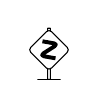
\begin{tikzpicture}[baseline=(x.base)]
		\draw[rounded corners=.01em] (-.05em,-1.07em)rectangle(.05em,.78em);
		\draw[fill=white,rounded corners=1.3] (0,.75em)--(.75em,0)--(0,-.75em)--(-.75em,0)--cycle;
		\draw[line width=0.2mm, line cap=round](-.4em,-1.07em)--(.4em,-1.07em);
		\node(x) at (0,0em) {};
		% Thank you https://tex.stackexchange.com/a/262510
		\draw[
			line cap=but,
			line join=round,
			x=.5em,
			line width=0.5mm,
			y=1*(height("Z")-\pgflinewidth)*(1-sin(10)),
			rotate=-10,
			rounded corners=1.5pt,
		](-0.57, 0.57) -- (0.57, 0.57) -- (-0.57, -0.57) -- (0.57, -0.57);
	\end{tikzpicture}%
}
\makeatletter
\declaretheorem[
	style=nirredbox,
	name=Idea,
	sibling=thm,
	% without \leavevmode, the first item in a list gets misformatted
	postheadhook={\leavevmode\marginnote{\nirideasymbol}[-3pt]%
	\ifthmt@thisistheone% restatable makes alignment weird
		\hspace{-2.2pt}%
	\fi}
]{idea}

\declaretheorem[
	style=nirredbox,
	name=Warning,
	sibling=thm,
	% without \leavevmode, the first item in a list gets misformatted
	postheadhook={\leavevmode\marginnote{\nirwarnsymbol}[-3pt]%
	\ifthmt@thisistheone% restatable makes alignment weird
		\hspace{-2.2pt}%
	\fi}
]{warn}
\makeatother

\title{Functional Analysis
\\ 
\vspace{0.4cm}
\large Fall 2025}




\date{\today}
\author{Hui Sun}


\begin{document}

\maketitle

\chapter{Preliminary}

\section{9/3 lecture}



\begin{defn}[orthonormal basis]
    Let $S$ be an orthonormal set in the Hilbert space such that no other orthonormal set contains $S$ as a proper subset. Then $S$ is called an orthonormal basis.
\end{defn}

\begin{prop}
    Every Hilbert space admits an orthonormal basis.
\end{prop}
\begin{proof}
    Zorn's lemma.
\end{proof}
Remark: if $H$ is separable, i.e., $H$ has a countable dense subset, then the proof does not require Zorn's lemma. For example, $L^2$ is separable.

\begin{prop}[II.6, Parsevel's formula]
    Let $\mathcal{H}$ be a Hilbert space, and $S=\{x_n\}$ be an orthonormal basis, then for each $y\in\mathcal{H}$, 
    \begin{equation*}
        y=\sum_{\alpha\in\mathcal{A}}(x_\alpha,y)x_\alpha, \quad \|y\|^2=\sum|(x_n,y)|^2
    \end{equation*}
    where $\mathcal{A}$ is an index set.
\end{prop}
\begin{proof}
    Bessel's inequality states that for any $\mathcal{A}'\subset\mathcal{A}$ finite, we have 
    \begin{equation*}
        \sum_{\alpha\in\mathcal{A}'}|(x_\alpha,y)|^2\leq\|y\|^2<\infty
    \end{equation*}
    It follows that $|(x_\alpha,y)|>\frac{1}{n}$ for at most finitely many $\alpha$'s, and $|(x_\alpha,y)|\neq 0$ for at most countably many $\alpha$'s. Let $\{\alpha_i\}_{i=1}^\infty$ be an enumeration of such $\alpha$'s. Then 
    \begin{equation*}
        \sum_{i=1}^N|(x_{\alpha_i},y)|^2\leq\|y\|^2<\infty
    \end{equation*}
    which implies 
    \begin{equation*}
        \sum_{i=1}^\infty|(x_{\alpha_i},y)|^2<\infty
    \end{equation*}
    Let 
    \begin{equation*}
        y_n=\sum_{i=1}^n(x_{\alpha_i},y)x_{\alpha_i}, 
    \end{equation*}
    we would like to show that the sequence $\{y_n\}$ is cauchy, 
    \begin{equation*}
        \|y_n-y_m\|^2=\left\|\sum_{i=m+1}^n(x_{\alpha_i}, y)x_{\alpha_i}\right\|^2\to 0 \text{ as } m\to\infty
    \end{equation*}
    Thus $\{y_n\}$ is Cauchy. In other words,
    \begin{equation*}
        y_n\to y=\sum_{i=1}^\infty (x_{\alpha_i},y)x_{\alpha_i}
    \end{equation*}
\end{proof}


\begin{defn}
    A metric space is separable if it has a countable dense subset.
\end{defn}

\begin{prop}[II.7]
    Let $\mathcal{H}$ be a Hilbert space, then it is separable iff it has a countable orthonormal basis.
\end{prop}
\begin{proof}
    Suppose $\mathcal{H}$ is separable, let $\{x_n\}$ be a countable dense set, then we throw out terms in $\{x_n\}$ until we get a linearly indepedent dense subset $\{u_n\}\subset \{x_n\}$. Applying Gram-Schmidt, we can assume $\{u_n\}$ to be countable and orthonormal. Conversely, if $\{u_n\}$ is a countable orthonormal basis, then the set of linear combinations of $\{u_n\}$ with rational coefficients forms a countable dense subset of $\mathcal{H}$.
\end{proof}



\begin{defn}[Fourier Coefficient]
    The $n$th Fourier coefficient of a $2\pi$-periodic function $f$ is 
    \begin{equation*}
        c_n=\frac{1}{\sqrt{2\pi}}\int_0^{2\pi}e^{-inx}f(x)dx
    \end{equation*}
    The Fourier series of $f$ is 
    \begin{equation*}
        \tilde{f}(x)=\lim_{M\to\infty}
        \sum_{M=-N}^N\frac{1}{\sqrt{2\pi}}c_ne^{inx}
    \end{equation*}
\end{defn}

\begin{prop}
    The Fourier series $\sum_{k}c_k$ converges if $f\in L^2$. Moreover, the series converges uniformly to a continuous function if $\sum|c_k|<\infty$ 
\end{prop}
I am too lazzy to type it up, but it uses the fun lemma below:
\begin{lem}
    Suppose $f$ is $2\pi$-periodic, and $(f, e^{inx})=0$ for all $n$, then $f\equiv 0$. (In other words, if all the Fourier coefficients are $0$, then the function must be identically zero).
\end{lem}


\section{9/8 Lecture}
\begin{defn}[Banach space]
    A complete normed linear space is called a Banach space.
\end{defn}
\begin{example}
    \begin{enumerate}
        \item $L^\infty(\R)=\{f:f(x)\leq M \text{ a.e. }\}$, where $\|f\|_\infty$ is the smallest such $M$, is a Banach space.
        \item Let $C(\R)$ be the bounded continuous functions on $\R$. Let $C(\R)\subset L^\infty(\R)$ and equip it with the same norm. Moreover, $C(\R)$ is also a Banach space (due to the uniform convergence of continuous functions is still continuous).
        \item Let $C_c(\R)$ be the space of continuous functions with compact support, and this is not a Banach space under $\|\cdot\|_\infty$.
        \item $L^p$ is complete for all $1\leq p<\infty$.
        \item Let $a=\{a_n\}$ be a sequence of complex numbers, ad 
        \begin{equation*}
            \|a\|=\sup_n|a_n|<\infty
        \end{equation*}
        let $c_0=\{\lim_{n\to\infty}a_n=0\}$, $s=\{\lim_{n\to\infty}n^Na_n=0 \forall N\}$, and $l_p=\{\|a\|_p^p=\sum_{n=1}^\infty|a_n|^p<\infty\}$. Note that the space 
        \begin{equation*}
            f=\{a_n=0 \text{ for al but finitely many $n$}\}
        \end{equation*}
        is not complete! However, it is a dense subset in $l^p$. Morever, the set of elements in $f$ with rational coefficients, and the closure of $f$ in $s, l^p, c_0$ are exactly the whole spaces, i.e., $s,l^p, c_0$ are separable.
        \item Let $L(X,Y)$ be bounded linear operators from $X,Y$, with the operator norm, and $L(X,Y)$ is a Banach psace.
    \end{enumerate}
\end{example}

\begin{prop}
    Let $L^p(\R)$, where $1\leq p<\infty$ be the space of functions with the norm 
    \begin{equation*}
        \|f\|_p=\left(\int_\R|f(x)|^pdx\right)^p
    \end{equation*}
    then 
    \begin{enumerate}
        \item (Minkowski's inequality) $\|f\|_p\leq\|f\|_p+\|g\|_p$.
        \item (Riesz-Fischer) $L^p$ is complete.
        \item (Holder) Given $\frac{1}{p}+\frac{1}{q}=\frac{1}{r}$, we have 
        \begin{equation*}
            \|fg\|_r\leq\|f\|_p\|g\|_q
        \end{equation*}
        if $f\in L^p, g\in L^q$.
    \end{enumerate}
\end{prop}


\begin{prop}
    If $Y$ is complete, then $L(X,Y)$ is a Banach space.
\end{prop}
\begin{proof}
    Suppose $\{A_n\}$ is Cauchy, now we construct the limit: for each $x$, $A_nx=y_n$ is a Cauchy sequence:
    \begin{equation*}
        \|y_n-y_m\|\leq\|A_n-Am\|\cdot\|x\|
    \end{equation*}
    Now since $Y$ is complete, we know that $A_nx\to y$. Let $Ax=y$. (This is our limit)! Now $\|A_n\|\leq C$ for all $n$, which implies $\|A\|\leq C$. Thus $L(X,Y)$ is complete!
\end{proof}

\subsection{Duals}
\begin{defn}[dual space]
    The space of bounded linear functionals $L(X,\C)$, where $X$ is Banach, is called the dual space to $X$, denoted by $X^*$. Let $f\in X^*$, then define the norm 
    \begin{equation*}
        \|f\|=\sup_{x\in X, \|x\|\leq 1}|f(x)|
    \end{equation*}
\end{defn}


\begin{example}
    \begin{enumerate}
        \item Suppose that $1<p<\infty$, $\frac{1}{p}+\frac{1}{q}=1$, and let $g\in L^q$, then 
        \begin{equation*}
            G(f)=\int_{-\infty}^\infty\bar{g}(x)f(x)dx
        \end{equation*}
        Then $G$ is in $(L^p)^*$. Moreover, any such linear functional on $L^p$ can be written in this way for some $g\in L^q$. And 
        \begin{equation*}
            |G(f)|\leq\|f\|_p\|g\|_q
        \end{equation*}
        by Holder. Moreover, 
        \begin{equation*}
            L^q(\R)^*=L^p, (L^q(\R)^*)^*=L^q
        \end{equation*}
        because $L^q$ is reflexive! In particular, $L^2$ is its own dual space.
        \item Suppose $\{\lambda_k\}\subset l^q$, then 
        \begin{equation*}
            \Lambda(\{a_k\})=\sum_k\lambda_ka_k
        \end{equation*}
        is a bounded linear functional on $l^p$. Thus 
        \begin{equation*}
            l_q\subset (l^p)^*
        \end{equation*}
    \end{enumerate}
    for $1\leq p\leq\infty$. It turns out every linear functional on $l^p$ can be written in this form.
\end{example}
\begin{example}
    Let $p=1$, we have 
    \begin{equation*}
        L^1(\R)^*=L^\infty, \text{ but } L^\infty(\R)^*\neq L^1(\R)
    \end{equation*}
    in fact $L^\infty(\R)^*$ is bigger. 
\end{example}



\section{9/10 Lecture}

\begin{prop}[Geometric Hahn-Banach]
    Let $V_1$ be a subspace of $V$, $x\in V\setminus V_1$, then one can find a hyperplane (codim $1$) $V_2$ such that $V_1\subset V_2$, and $x\not\in V_2$. 
\end{prop}
\begin{proof}
    If $V_1$ has codim$V_1=1$, then we are done. Suppose that codim $V_1>1$, we would like to find $V_2$ such that $x\not\in V_2$, where $V_2\neq V_1$ such that $\dim(V/V_1)>1$. Note that we define 
    \begin{equation*}
        \dim(V/V_1)=\{[z]: [z]=[w] \iff z+w\in V_1\}
    \end{equation*} 
    (For any banach space, we can write $B=W\oplus(B/W))$. This implies that we can find $y=[y]\in V/V_1$ such that $y\not0$, and $y\neq x$ (by codim $>1$). Set 
    \begin{equation*}
        V_2=\{z+ty; z\in V_1, t\in\R\}
    \end{equation*}
    Then we can continue this process, and using Zorn's lemma, we can have $V_2$ to have codim $1$.
\end{proof}

\begin{defn}
    A subset $A\subset V$ is called  if for any $x,y\in V$, the line connecting them is contained in $A$. If the set is also open, then we call $A$ convex linearly open.
\end{defn}

\begin{prop}[Geometric HB for Convex sets]
    Let $A\subset V$ be convex linearly open, and let $V_1$ be a linear subspace which does not intersect $A$. Then there is a hyperplane  $V_2$ such that $V_1\subset V_2$ and $V_2\cap A=\emptyset$.
\end{prop}
(Essentially proof by picture).
% \begin{proof}
%     Suppose that $\dim V=2$, and $\dim (V_1)=0$. (Convexity is important! Consider a nonconvex donut around a line). Consider 
% \end{proof}


\begin{prop}[Hahn-Banach]
    Let $X$ be a real vector space, for all $x,y\in X$, and $\alpha\in[0,1]$, with sublinear functional $p(x)$ satisfying 
    \begin{equation*}
        P(\alpha x+(1-\alpha)y)\leq\alpha p(x)+(1-\alpha)p(y)
    \end{equation*}
    Suppose that $\lambda$ is a linear functional  defined on a subspace on $Y$ such that $\lambda(y)\leq p(y)$ for all $y\in Y$. Then there is a linear functional $\Lambda$ on $X$ such that $\Lambda=\lambda$ on $Y$, and 
    \begin{equation*}
        \Lambda(x)\leq p(x)
    \end{equation*}
\end{prop}
\begin{proof}
    Let $x\in Y\setminus Y$, we will first show that we can extend $\lambda$ to the subspace spanned by $Y$ and $z$, following the same bound. Define 
    \begin{equation*}
        \tilde{\lambda}(az+y)=a\tilde{\lambda}(z)+\lambda(y)
    \end{equation*}
    Suppose that $y_1,y_2\in Y$, and $\alpha,\beta>0$, and 
    \begin{align*}
        \beta\lambda(y_1)+\alpha\lambda(y_2)=\lambda(\alpha y_1+\beta y_2)&=(\alpha+\beta)\lambda\left(\frac{\beta}{\alpha+\beta}y_1+\frac{\alpha}{\alpha+\beta}y_2\right)\\
        &\leq(\alpha+\beta)p(\dots)\\
        &\leq\beta p(y_1-\alpha z)+\alpha(y_2+\beta z)
    \end{align*}
    deviding both sides by $\alpha,\beta$, taking the sup over $\alpha>0, y$, we see that 
    \begin{equation*}
        \tilde{\lambda}(x)\leq p(x)
    \end{equation*}
    for all $x$ in this subspace. Using Zorn's lemma, we extend one subspace at a time, then we are done.
\end{proof}




\section{9/15 Lecture}
\begin{prop}[Geometric Hahn-Banach]
    Let $A$ be complex and linearly open, and $A\subset V$ be a vector space over $\R$. Let $V_1$ be a subspace of $V$, $V_1\cap A=\emptyset$. Then there exists a hyperplane $V_2$ such that $V_2\cap A=\emptyset, V_1\subset V_2$. 
\end{prop}

\begin{defn}
    A seminorm $p$ is such that $p(x)\geq 0, p(x+y)=p(x)+p(y)$, and $p(\alpha x)=|\alpha|p(x)$.
\end{defn}

And we have the following analytic version of Hahn-Banach.
\begin{prop}[Analytic Hahn-Banach]
    Let $W$ be a subspace of $V$, and $f$ linear form on $W$ such that $|f(x)|\leq p(x)$, for all $x\in W$. Then there is a linear form $f_1$ such that $f_1(x)=f(x)$ on $W$, and $|f_1(x)|\leq p(x)$ for all $x$.
\end{prop}
I am too lazy to follow the proof.
% \begin{proof}
%     Let $W$ be the affine subspace, $\{x\in W: f(x)=1\}$. Then $W_1$ does not meet the set $A=\{x\in V: p(x)<1\}$. By the geometric Hahn-Banach, there is a hyperplane $V_1=\{x\in V: f_1(x)=1\}$, which constains $W_1$ and does not intersect $A$. (For $x_1\in W_1$, let $W_1'=W_1-x_1, A'=A-x_1$, which gives $V_1'=V_1-x_1$).
% \end{proof}

\section{9/17 Lecture}

\begin{prop}
    Let $T:X\to Y$ be a linear map, $T$ is bounded iff 
    \begin{equation*}
        T^{-1}(\{y: \|y\|\leq 1\})
    \end{equation*}
    has nonempty interior. 
\end{prop}
\begin{proof}
    Suppose that it has a nonempty interior, then 
    \begin{equation*}
        \{x: \|x-x_0\|\leq\varepsilon\}\subset T^{-1}(\{y: \|y\|\leq 1\})
    \end{equation*}
    Then if $\|x\|\leq\varepsilon$, then 
    \begin{equation*}
        \|Tx\|\leq\|T(x-x_0)\|+\|Tx_0\|\leq 1+\|Tx_0\|
    \end{equation*}
    then 
    \begin{equation*}
        T\left(\frac{\varepsilon x}{\|x\|}\right)=\frac{\varepsilon}{\|x\|}T(x)\Rightarrow \|T(x)\|\leq(1+\|Tx_0\|)\frac{1}{\varepsilon}\|x\|
    \end{equation*}
\end{proof}

\begin{defn}[nowhere dense]
    A set $S$ is called nowhere dense if $\overline{S}$ has empty interior.
\end{defn}

\begin{prop}[Baire category theorem]
    A complete metric space $M$ is never a union of a countable number of nowhere dense sets.
\end{prop}
\begin{proof}
    Suppose $M=\bigcup_{n=1}^\infty A_n$, where $A_n$ is nowhere dense. We will construct $\{x_n\}$ that stays away from each $A_n$ so the limit $x$ is in any $A_n$, which gives a contradiction. Take $x_1\in\bar{A}_1$, and $B_1\cap A_1=\emptyset$, and $B_1=B(x_1,r_1)=\{d(x,x_1)<\varepsilon\}$, let $x_2\in B_1\setminus A_1$, and let $B_2=B(x_2, r_2)$, and so on, $\{x_n\}$ is a Cauchy sequence, $x_n\to x$ as $n\to\infty$. We have $x_n\in B_N, n\geq N$, but $\bar{B}_N\subset B_{N-1}$, thus $x\in B_{N-1}$ for any $N$, and $x\not\in A_{N-1}$ for any $N$. This gives our contradiction.
\end{proof}

\begin{prop}[UBP]
    Let $X$ be a Banach space, let $\mathcal{F}$ be a family of bounded linear maps $T: X\to Y$. Suppose that for each $x\in X$,
    \begin{equation*}
        \left\{\|Tx\|: T\in\mathcal{F}\right\}
    \end{equation*}
    is bounded, then
    \begin{equation*}
        \sup_{T\in\mathcal{F}}\|T\|<\infty
    \end{equation*}
\end{prop}
\begin{proof}
    Key ingredient: Baire category theorem. Let $B_n=\{x: \|Tx\|\leq n, T\in\mathcal{F}\}$, each $x$ is in some $B_n$, and $X=\bigcup_{n=1}^\infty B_n$, where $B_n$ is closed. Baire category theorem, some $B_n$ has nonempty interior. 
    \begin{equation*}
        B_n\{x: \|Tx\|\leq n\}\Rightarrow \{|x: \|Tx\|\leq 1\}
    \end{equation*}
    And 
    \begin{equation*}
        \|Tx\|\leq(1+\|Tx_0\|)\|x\|\Rightarrow \|T\|\leq 1+\|T(x_0)\|
    \end{equation*}
\end{proof}

% An immediate corollary is the following:
% \begin{prop}
%     Let $X,Y$ be Banach spaces, let $B(\cdot, \cdot)$ be separately continuous on $X,Y$, then 
%     \begin{equation*}
%         B: X\times Y\to \mathbb{C}
%     \end{equation*}
%     is jointly continuous. If $x_n\to x, y_n\to y$, then $B(x_n,y_n)\to B(x,y)$.
% \end{prop}

\section{9/22 Lecture}
\begin{defn}[homeomorphism]
    Let $f:S\to T$, be a map between two topological spaces, then $f$ is called a homeomorphism if it is a continuous bijection with a continuous inverse.
\end{defn}

\begin{defn}
    Let $K$ be a family of functions $f: S\to (\tau, \tau_U)$, then $X$ is the weak topology on $S$ if it is the weakest topology making all $f\in K$ continuous: for any $U\in \tau_U$, $f^{-1}(U)$ is open in $X$. 
\end{defn}

\begin{example}
    Let $\mathcal{H}$ be a Hilbert space. Then the weak topology on $\mathcal{H}$ is the weakest topology that makes 
    \begin{equation*}
        \varphi\mapsto\la\varphi,\psi\ra
    \end{equation*} 
    continuous for each $\psi\in\mathcal{H}$.
\end{example}



\begin{defn}[Hausdorff]
    A topological space is called Hausdorff iff for each $x\neq y$, there exists open sets $U_1, U_2$ such that $x\in U_1, y\in U_2$ and $U_1\cap U_2=\varnothing$/. A topological space is called 
    \begin{enumerate}
        \item separable if it contains a countable dense subset.
        \item first countable if each point has a countable neighborhood base. 
        \item second countable iff it has a countable base.
    \end{enumerate}
    We note that every metric space is first countable, and is second countable if it is separable. Finally, any second countable space is separable.
\end{defn}


Now we talk about some nets.
\begin{defn}[directed system, net]
    A directed system is an index set $I$ together with an ordering $\prec$ such that 
    \begin{enumerate}
        \item $\alpha,\beta\in I$, there is $\gamma\succ\alpha, \gamma\succ\beta$.
        \item there is a partial ordering.
    \end{enumerate}
    A net on a set $S$ is a mapping $I: A\mapsto x_A\in S$ such that $\{x_\alpha\}_{\alpha\in I}$. If $I$ is positive integers then the nets are just sequences $\{x_i\}_{i=1}^\infty$.

    A net $\{x_\alpha\}_{\alpha\in I}$ is said to converge to $x\in S$ if for any neighborhood $N$ of $x$, there is $\beta\in I$ so $x_\alpha\in N$ if $\alpha\succ\beta$.
\end{defn}

\begin{prop}
    A function $f: S\to T$ is continuous iff for eery convergent net $\{x_\alpha\}$, the net $\{f(x_\alpha)\}$ converges too. (If $S,T$ are first countable, then the nets can be taken as sequences).
\end{prop}
Then we defined compact and FIP for topological spaces, and claimed that they are equal.

\begin{example}
    The unit ball in $l_2$ is not compact.
\end{example}

\begin{prop}[Tychnoff]
    An arbitrary product of compact topological spaces is compact.
\end{prop}

\begin{prop}[Stone-Weierstrass]
    Let $B$ be a subalgebra of $C_\R(X)$, where $X$ is Hausdorff, compact that separates points, i.e., if $x\neq y$, this implies $f(x)\neq f(y)$ for some $f\in B$ and $L\in B$, then $B=C_\R(X)$.
\end{prop}




\begin{example}
    Let $B$ be the closure of the set $\{e^{ikx}\}_{k=-\infty}^\infty$, on $[-\pi,\pi]$. Then by Stone Weierstrass, we must have $B=C[-\pi,\pi]$.
\end{example}


% Harmonic analysis lecture
% \section{Lecture 9/22 Harmonic!}
% We will prove the following Strichartz estimates:
% last time we did
% \begin{equation*}
%     \int_{\R^n}|\hat{F}(\xi,|\xi|)|^2\frac{d\xi}{|\xi|}\lesssim\|F\|_{L^\frac{2(n+1)}{n+3}(\R^{n+1})}
% \end{equation*}
% for any $f\in\mathcal{S}$. And similarly, we will show 
% \begin{equation}\label{1}
%     \int_{\R^n}|\hat{F}(\xi,|\xi|^2)|^2\frac{d\xi}{|\xi|}\lesssim\|F\|_{L^\frac{2(n+2)}{n+4}(\R^{n+1})}
% \end{equation}


% \begin{prop}[Stein-Tomas]
%     Case of $(\mathbb{S}^{n-1})$: 
%     \begin{equation*}
%         \left(\int_{\mathbb{S}^{n-1}}|\hat{F}(\omega)|^2d\omega\right)^\frac{1}{2}\leq c\|F\|_{L^\frac{2(n+1)}{n+3}}
%     \end{equation*}
%     and for any $L^r$ where $1\leq r\leq\frac{2(n+1)}{n+3}$.
% \end{prop}


% We recall that the solution to the Scrodinger's equation $\frac{1}{i}\partial_tu=\Delta f$, where $u(t=0)=0$,
% \begin{equation*}
%     u=(e^{-it\Delta}f)(x)=\int_{\R^n}e^{ix\cdot\xi+it|\xi|^2}\hat{f}(\xi)d\xi\coloneq (Tf)(x,t)
% \end{equation*}
% The process of beginning with $n$ variables and turning into $n+1$ variables is why we call this Fourier extension. (On the other hand, the Strichartz estimate is Fourier restriction).

% The above is equivalent to the following estimate:
% \begin{equation*}
%     \|u\|_{L^\frac{2(n+2)}{n}(\R^{n+1})}\leq CC\|f\|_{L^2(\R^n)}
% \end{equation*}
% i.e., 
% \begin{equation*}
%     \|Tf\|_{L^\frac{2(n+2)}{2}(\R^{n+1})}\leq C\|f\|_{L^2(\R^n)}
% \end{equation*}
% We now show that this is equivalent to Equation\ref{1}. We consider the dual $T^*$, and by the $TT^*$ method, it suffices to show that 
% \begin{equation*}
%     \|TT^*G\|_{L^\frac{2(n+2)}{n}_{t,x}}\leq \|G\|_{L_{t,x}^\frac{2(n+2)}{n+4}}
% \end{equation*}
% % \begin{equation*}
% %     \|Tf\|_{L^\frac{2(n+2)}{n}}\leq C\|f\|_{L^2(\R^n)}
% % \end{equation*}
% where 
% \begin{align*}
%     TT^*G(x,t)&=\int_s\int_y\int_\xi e^{i(x-y)\cdot\xi+i(t-s)|\xi|^2}G(y,x)d\xi dyds\\
%     =\int K(x,t,y,x)G(y,x)dyds
% \end{align*}
% where 
% \begin{equation*}
%     K(x,t,y,x)=\int_{\R^n}e^{i(x-y)\cdot\xi+\i(t-s)|\xi|^2}d\xi
% \end{equation*}
% It is enough (just like the cone) to prove it for dyadic pieces, where 
% \begin{equation*}
%     K(x,t,y,s)=\int_{\R^n}e^{i(x-y)\cdot\xi+i(t-s)|\xi|^2}\beta(|\xi|)d\xi
% \end{equation*}
% and 
% \begin{equation*}
%     |K|\lesssim |t-s|^{-\frac{n}{2}}
% \end{equation*}
% Now we consider the freezing operators 
% \begin{align*}
%     (W_{t,s}f)(x)&=\int_{\R^n}K(x,t,y,s)f(y)dy\\
%     &=\int\int e^{i(x-y)\cdot\xi+i(t-s)|\xi|^2}\beta(|\xi|)f(y)d\xi dy
% \end{align*}
% thus 
% \begin{equation*}
%     \|W_{t,s}\|_{L_x^\frac{2(n+2)}{n+4}\to L_x^\frac{2(n+2)}{2}}=O\left(|t-s|^\frac{-2}{q}\right)
% \end{equation*}

% Let's now prove the Stein-Tomas estimate:
% Let $\Sigma$ be a hypersurface with nonvanishing curvature; but by a partition of unity argument, 
% \begin{equation*}
%     \Sigma=\left\{(\xi', h(\xi')):\xi'\in\R^{n-1}\right\}
% \end{equation*}
% we want to show that 
% \begin{equation*}
%     \left(\int|\hat{F}(\xi', h(\xi'))a(\xi')^{1/2}|^2d\xi'\right)^\frac{1}{2}\leq C\|F\|_{L^r(\R^n)}
% \end{equation*}
% where 
% \begin{equation*}
%     Tf(x',x_n)=\int_{\R^{n-1}}e^{ix'\cdot\xi'+ix_nh(\xi')}(a(\xi'))^\frac{1}{2}f(\xi')d\xi'
% \end{equation*}
% and 
% \begin{equation*}
%     T^*F(\xi')=\hat{F}(\xi',h(\xi'))(a(\xi'))^\frac{1}{2}
% \end{equation*}
% Note $T^*: L^r(\R^n)\to L^2(\R^{n-1})$, and $T:L^2(\R^{n-1})\to L^{r'}(\R^n)$., and 
% \begin{equation*}
%     TT^*: L^r(\R^n)\to L^{r'}(\R^n)
% \end{equation*}
% and 
% \begin{equation*}
%     WF(x)=TT^*F(x)=\int\int e^{i(x'-y')\cdot\xi'+i(x_n-y_n)h(\xi')}G(y', y_n)a(\xi')d\xi'dy'dy_n
% \end{equation*}
% this is the exact same case now, where 
% \begin{equation*}
%     K=\int e^{i(x'-y')\cdot\xi'+i(x_n-y_n)h(\xi')}a(\xi')d\xi'=O(|x_n-y_n|^{-\frac{n-1}{2}})
% \end{equation*}
% i.e., 
% \begin{equation*}
%     \|W_{x_n,y_n}\|_{L^1\to L^\infty}=O(|x_n-y_n|^{-\frac{n-1}{2}})
% \end{equation*}
% and 
% \begin{equation*}
%     \|W_{x_n,y_n}\|_{L^2\to L^2}=O(1)
% \end{equation*}
% thus $W=TT^*$, we have $W: L^r(\R^n)\to L^{r'}(\R^n)$. We have now proven Stein-Tomas.



\section{Lecture 9/24}
\begin{prop}[Riesz-Markov]
    Let $X$ be compact and Hausdorff, then for any positive linear functional $l$ on $C(X)$, there is a unique Baire measure $\mu$ such that 
    \begin{equation*}
        l(f)=\int fd\mu
    \end{equation*}
    For example, let $X=[-1,1]$, let $l(f)=f(0)$, then $\mu=\delta_0$. This means that you can continuously extend $l$ so that it is defined on characteristic functions on Baire sets.
\end{prop}
% \begin{proof}
%     A function with values in $(-\infty,\infty]$ is called lower semicontinuous if $\{x: f(x)>a\}$ are open. Let $I^+$ be the nonnegative lower semi-continuous functions. Then $h\in I^+$ is the limit from below of functions in $C_0$. Thus we define 
%     \begin{equation*}
%         l^*(h)=\sup_{h\geq g\in C_0}l(g)
%     \end{equation*}
%     for general $f\geq 0$, define $l^*(f)=\inf_{f\leq h\in I^*}l^*(h)$. We say $f\in L_l^1$ if for each $\varepsilon>0$, there is $g\in C_0$ so $l^*(|f-g|)<\varepsilon$, define 
%     \begin{equation*}
%         l(f)=\lim l(g_n)
%     \end{equation*}
%     and $g_n\in C_0$, and $l^*(|f-g_n|)\to 0$. The functional $l^*$ is calle da Radon measure. Let $l$ be a Radon measure on $(a,b)$, we will show that $l$ is the Riemann-Stieltjes integral 
%     \begin{equation*}
%         l(f)=\int fd\phi
%     \end{equation*}
%     with respect to a nondecreasing function $\phi$, 
%     \begin{equation*}
%         \sum f(x_i)[\phi(x_{i+1})-\phi(x_i)]
%     \end{equation*}
%     Let $m_k=\min_{x\in I_k}f(X), M_k=\max_{x\in I_k}f(x), I_k[x_k, x_{k+1}]$. Let 
%     \begin{equation*}
%         H_x(y)=\begin{cases}
%             1, y>x\\
%             0, y\leq x
%         \end{cases}
%     \end{equation*}
%     i.e., $H_{x_1}-H_{x_2}\in L_l^1$. Up to a constant, there is a unique $\phi$ such that $\phi(x_2)-\phi(x_1)=\mu$, 
%     \begin{equation*}
%         \phi(x_2)-\phi(x_1)=l^*(H_{x_1}-H_{x_2})
%     \end{equation*}
%     and 
%     \begin{equation*}
%         \phi(x_2)-\phi(a)-[\phi(x_1)-\phi(a)]=l^*(H_{x_1}-H_a)-l^*(H_{x_2}-H_a)
%     \end{equation*}
%     This menas that $\phi$ is nondecreasing. Notice 
%     \begin{equation*}
%         \sum m_k(H_{x_k}-H_{x_{k+1}})\leq f(x)\leq \sum M_k(H_{x_k}-H_{x_{k+1}})
%     \end{equation*}
%     Then 
% \end{proof}



\begin{defn}[weak topology]
    The weak topology on $X$ is the weakest topology that make each $l\in X^k$ continuous. A sequence converges weakly $x_n\xrightarrow{w} x$ iff $l(x_n)\to l(x)$ for all $l\in X^*$.
\end{defn}



\begin{prop}
    We have the following properties:
    \begin{enumerate}
        \item The weak topology is weaker than the norm topology.
        \item For weakly convergent s sequence is norm bounded.
        \item The weak topology is Hausdorff.
    \end{enumerate}
\end{prop}
\begin{example}
    Let $\mathcal{H}$ be a Hilbert space, and $\{\varphi_\alpha\}$ an orthonormal base. Given $\psi_n$ a sequence in $\mathcal{H}$. And 
    \begin{equation*}
        \varphi_n^{(a)}=(\psi_n,\varphi_\alpha)
    \end{equation*}
    where $\psi_n=\sum\psi_n^{(a)}\varphi_\alpha$, then 
    \begin{equation*}
        \psi_nx\xrightarrow{w}\psi
    \end{equation*}
    iff $\psi_n^{(a)}\to\psi^{(a)}$ and $\{\|\psi_n\|\}$ is bounded. 
\end{example}

\begin{prop}
    A linear functional $l$ on a Banach space is weakly continuous iff it is norm continuous.
\end{prop}














\end{document}